\documentclass[journal,12pt,twocolumn]{IEEEtran}
\usepackage{cite}
\usepackage{amsmath,amssymb,amsfonts,amsthm}
\usepackage{algorithmic}
\usepackage{graphicx}
\usepackage{textcomp}
\usepackage{xcolor}
\usepackage{txfonts}
\usepackage{listings}
\usepackage{enumitem}
\usepackage{mathtools}
\usepackage{gensymb}
\usepackage{comment}
\usepackage[breaklinks=true]{hyperref}
\usepackage{tkz-euclide} 
\usepackage{textgreek}                       
\usepackage{circuitikz}
\usepackage{pgfplots}                            
\usepackage[latin1]{inputenc}                                
\usepackage{color}                                            
\usepackage{array}                                            
\usepackage{longtable}                                       
\usepackage{calc}                                             
\usepackage{multirow}                                         
\usepackage{hhline}                                           
\usepackage{ifthen}                                           
\usepackage{lscape}

\newcommand{\brak}[1]{\left[#1\right]}

\newtheorem{theorem}{Theorem}[section]
\newtheorem{problem}{Problem}
\newtheorem{proposition}{Proposition}[section]
\newtheorem{lemma}{Lemma}[section]
\newtheorem{corollary}[theorem]{Corollary}
\newtheorem{example}{Example}[section]
\newtheorem{definition}[problem]{Definition}
\newcommand{\BEQA}{\begin{eqnarray}}
\newcommand{\EEQA}{\end{eqnarray}}
\newcommand{\define}{\stackrel{\triangle}{=}}
\theoremstyle{remark}
\newtheorem{rem}{Remark}

\begin{document}

\bibliographystyle{IEEEtran}
\vspace{3cm}

\title{NCERT 11.9.2 Q7}
\author{EE23BTECH11204 - Ashley Ann Benoy$^{*}$}% <-this % stops a space
\maketitle
\newpage
\bigskip
\bibliographystyle{IEEEtran}
\textbf{Question: Find the sum of n terms of the A.P. whose kth term is \(5k + 1\).}\\
\solution
\begin{table}[h!]
    \centering
    \resizebox{6cm}{!}{
        \textbf{
\begin{table}[htbp]
\centering
\caption{Given Data}
\label{tab:data}
\begin{tabular}{|c|c|c|}
\hline
\textbf{Symbol} & \textbf{Value} & \textbf{Parameter} \\
\hline
\(x(0)\) & \(1 \) & First Term \\
\hline
\(x(k)\) & \(5k + 1 \) & kth Term \\
\hline
\(d\) & \(5 \) & Common Difference \\
\hline
\(S(n)\) & \(?\) & Sum of \(N\) terms \\
\hline
\end{tabular}
\end{table}
}

    }
    \\
    \caption{Given Parameters}
    \label{tab:given_params}  
\end{table}

Apply the Z-transform to \( x\brak{n} \):
\begin{align}
X\brak{z} = \frac{5z^{-1}}{\brak{1 - z^{-1}}^2} + \frac{1}{\brak{1 - z^{-1}}}
\quad |z|>1
\end{align}

Sum of First \( n \) Terms:

\begin{align}
y\brak{n} = x\brak{n} * u\brak{n}
\end{align}

Applying Z transform on both sides:
\begin{align}
    Y\brak{z} &= X\brak{z}U\brak{z}
\end{align}

\begin{align}
&=\frac{1}{\brak{1 - z^{-1}}^2} + \frac{5}{2} \cdot \frac{2z^{-1}}{\brak{1 - z^{-1}}^3} 
\end{align}
\\
Now we can compare the  above pairs as;
\begin{align}
nu\brak{n} \xleftrightarrow{\text{Z}} \frac{z^{-1}}{(1 - z^{-1})^2}
\end{align}
\begin{align}
u\brak{n} \xleftrightarrow{\text{Z}} \frac{1}{(1 - z^{-1})}
\end{align}
\begin{align}
n\brak{n-1}u\brak{n} \xleftrightarrow{\text{Z}} \frac{2z^{-1}}{(1 - z^{-1})^3}
\end{align}
On referring the above equations and comparing, we can obtain the  Z transform inverse as follows:

\begin{align}
y\brak{n} = \brak{n+1 }u\brak{n} + \frac{5}{2} n\brak{n-1} u\brak{n}
\end{align}
Therefore we have got the sum of n terms as:
\begin{align}
y\brak{n}= \brak{n+1 + \frac{5}{2} n\brak{n-1}}u\brak{n}
\end{align}
The stem plot is given as
\begin{figure}[h!]
  \centering
  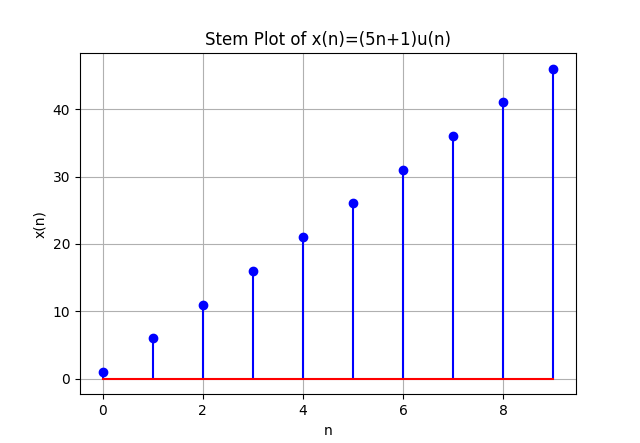
\includegraphics[width=\columnwidth]{figs/stem.png}
  \label{fig:Stem_Plot}
\end{figure}
\end{document}
